%%%%%%%%%%%%%%%%%%%%%%%%%%%%%%%%%%%%%%%%%%%%%%%%%%%%%%%%%%%%%%%%%%%%%%%%%
% Template for a classical article
%%%%%%%%%%%%%%%%%%%%%%%%%%%%%%%%%%%%%%%%%%%%%%%%%%%%%%%%%%%%%%%%%%%%%%%%%
\documentclass[12pt,a4paper,notitlepage,onecolumn]{article}
%%%%%%%%%%%%%%%%%%%%%%%%%%%%%%%%%%%%%%%%%%%%%%%%%%%%%%%%%%%%%%%%%%%%%%%%%
\newcommand{\Author}{Fabio Zanini}
\newcommand{\Title}{First modelling result}
%%%%%%%%%%%%%%%%%%%%%%%%%%%%%%%%%%%%%%%%%%%%%%%%%%%%%%%%%%%%%%%%%%%%%%%%%
\usepackage[english]{babel}
\usepackage[utf8x]{inputenc}
\usepackage{amsmath,amsfonts,amssymb,eucal,eurosym}
\usepackage{color}
\usepackage{graphicx}
\usepackage[font=small, format=hang, labelfont={sf,bf}, figurename=Fig.]{caption}
%\usepackage{cite}
%\usepackage{epigraph}
%\setlength{\epigraphwidth}{.55\textwidth}
%\setlength{\epigraphrule}{0pt}
%\usepackage{multirow}
%\usepackage[version=3]{mhchem}
%\usepackage{sagetex}
\usepackage[	colorlinks,linkcolor=red,citecolor=red]{hyperref}
\hypersetup{	pdfauthor={\Author}, pdftitle={\Title}, pdfkeywords={\Keywords}	}
%%%%%%%%%%%%%%%%%%%%%%%%%%%%%%%%%%%%%%%%%%%%%%%%%%%%%%%%%%%%%%%%%%%%%%%%%
\graphicspath{{./figures/}}
%%%%%%%%%%%%%%%%%%%%%%%%%%%%%%%%%%%%%%%%%%%%%%%%%%%%%%%%%%%%%%%%%%%%%%%%%
%\DeclareMathOperator\de{d\!}
%\newcommand{\comment}[1]{\textit{\textcolor{red}{#1}}}
%%%%%%%%%%%%%%%%%%%%%%%%%%%%%%%%%%%%%%%%%%%%%%%%%%%%%%%%%%%%%%%%%%%%%%%%%
\title{\Title}
\author{\Author}
\date{\today}
%%%%%%%%%%%%%%%%%%%%%%%%%%%%%%%%%%%%%%%%%%%%%%%%%%%%%%%%%%%%%%%%%%%%%%%%%
\begin{document}
\maketitle

\begin{figure}[h!]
 \begin{center}
  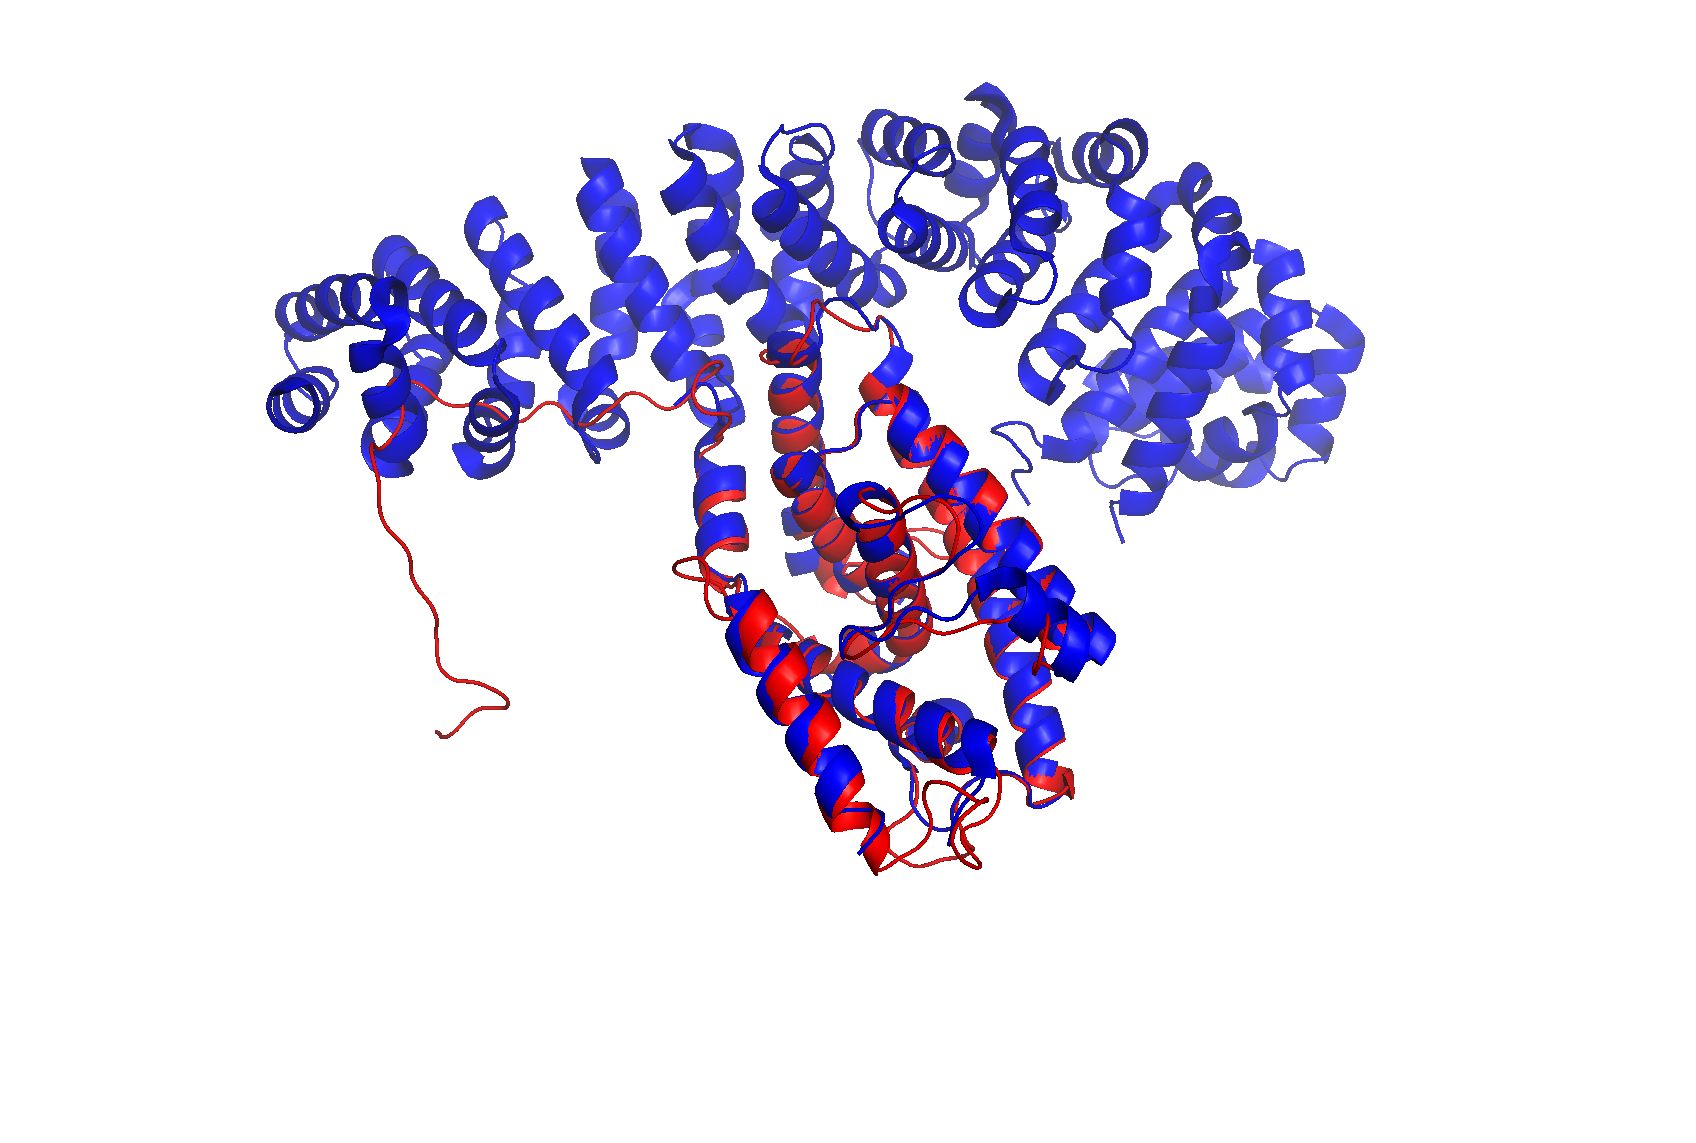
\includegraphics[width=0.8\linewidth]{1yje_A-3tx7_B.png}
  \caption{Example of a good model, our unknown sequence threaded onto 3XT7, chain B. Colors: red = our model, blue = 3XT7, chain B.}
  \label{fig:1yje_A-3xt7_B}
 \end{center}
\end{figure}
Taylor has written a skeleton script (\texttt{model\_align.py}) that does the modelling onto a single template. I have slightly expanded it to to several independent models onto single templates (\texttt{align\_model\_all.py}). A good example is shown in \figurename~\ref{fig:1yje_A-3xt7_B}.

Also, now we have all PDB entries in \texttt{data/templates/pdb}, so we can in principle do multi-template modelling.

\end{document}

